\chapter{A simulation study}\label{ch:simulation}

A careful reader may arrive at this chapter with a reasonable doubt. The earlier
chapters derived their results as propositions, with assumptions and proofs. A
simulation, on this view, can only confirm them. If the reciprocal of the key
frequency is the right risk under four assumptions, a simulation built on those
assumptions returns the reciprocal of the key frequency, and a simulation built on
other assumptions returns whatever those assumptions imply. Either way the formula
already knew the answer, and the computer time was spent on arithmetic. In its
strongest form the doubt adds that simulated populations are chosen by the
analyst, so a simulation that disagrees with a formula has shown only that the
analyst chose a population on which it disagrees.

The first fact that breaks the doubt comes from a release that satisfies the most
widely used rule in the field. On a synthetic population of 200,000 units with a
5 per cent sample, a release that is 10-anonymous on its declared key, so that no
released key class has fewer than ten members and the formula puts every record's
risk at or below 0.1, contains a record that the declared adversary identifies with
probability 0.744. Its one-sided 95 per cent lower bound, corrected for having
picked the worst of 230 records, is 0.638.
% source: paper/generated/table_kanonymity.tex (k=10: 230 targets, worst 0.744, bound 0.638); paper/generated/numbers.tex \runkanon10worst, \runkanon10worstlower
No formula in the earlier chapters produced that number. Proposition~\ref{prop:kanon}
said that the implication from $k$-anonymity to a risk of $1/k$ can fail once the
release publishes a continuous variable the adversary also reads. It did not say
whether the failure is a curiosity at the edge of the parameter space or a
property of an ordinary release. Only an attack run against a population whose
truth is known can say which.

This chapter asks one question. What does an attack simulated on a known
population show that the formulas cannot? The answer comes in five pieces: the
sizes of gaps the formulas only sign, the direction of effects the formulas leave
open, the behaviour of the worst record where formulas speak of averages, the
calibration of the adversary's own model, and the size of the programme effect of
Chapter~\ref{ch:programmes} at registers of different sizes.

\section{A file for a visiting researcher}

Tomás had asked the Bank for a research file of firm-level records: district,
size, age of the firm in years, sector, and a continuous measure of the firm's
borrowing. Naledi proposed to release it with a minimum class size of ten on the
four categorical fields. The chair asked why the assessment plan included a
simulated attack at all. A class size of ten meant a risk of at most one in ten,
she said, and that was the Bank's working tolerance for research files. Naledi
agreed that it meant one in ten under the formula. Her question was whether the
formula's assumptions held for a file that also published borrowing, which a
lender such as Pieter's would know, roughly, for its own customers.

The study in this chapter is the one Naledi would need to answer her own question,
built on a population where the answer is known. It is synthetic, its parameters
are chosen, and every result in it describes that population. Its value is that
every estimate can be compared with a truth, which is impossible on a real file
(Chapter~\ref{ch:public}).

\section{Design}

The population has $N = 200{,}000$ units. Each carries a district (40 categories
with a skewed size distribution), sex, age in single years from 18 to 87, and an
occupation group (12 categories, also skewed). District and occupation are drawn
with probabilities proportional to $j^{-0.9}$ and $j^{-0.8}$, and ages are thinned
towards younger values so that the oldest bands are sparse.
% source: paper/bis_ifc_full.tex, Section "Simulation study", Design, and Appendix "Simulation details"; artifacts-paper/config.json
The adversary's key is the cross-classification of district, sex, five-year age
band and occupation group. It has 13,440 possible cells, of which 12,596 are
occupied, and 1,305 cells are population unique, so 0.65 per cent of the
population would be identifiable from the key alone in a census.
% source: paper/generated/numbers.tex (\runcellspossible, \runcellsoccupied, \runpopulationuniquecells, \runpopulationuniqueshare)

Each unit also carries a confidential continuous variable,
\begin{equation}\label{c11:eq-y}
y_i = 8 + \psi_{d(i)} + \omega_{o(i)} + 0.018\,(\mathrm{age}_i - 50)
+ 0.10\,\mathrm{sex}_i + \epsilon_i ,\qquad \epsilon_i \sim N(0, 0.6^2),
\end{equation}
with district effects $\psi$ and occupation effects $\omega$ drawn once from
$N(0, 0.45^2)$ and $N(0, 0.35^2)$.
% source: paper/bis_ifc_full.tex, Section "Simulation study", Design
The variable plays the part of Tomás's borrowing measure, or of an income in a
household survey. A Bernoulli sample with inclusion probability $\pi = 0.05$ gives
$n = 10{,}035$ records with 4,679 distinct keys, of which 2,729 are unique, so 27.2
per cent of released records are sample unique.
% source: paper/generated/numbers.tex (\runreleased, \runreleasedcells, \runreleaseduniquecells, \runreleaseduniqueshare)

The declared adversary observes district and sex without error. It reads the
released age band with probability 0.15 of a one-band error and the occupation
group with probability 0.10 of a wrong group, and it holds a noisy reading
$z_t = y_t + N(0, 0.75^2)$ of the confidential variable.
% source: artifacts-paper/config.json (error_age 0.15, error_occupation 0.10, covariate_sd 0.75)
It links by maximum posterior, in the sense of \eqref{eq:maxpost} in
Chapter~\ref{ch:scenario}, under the same error model that generates its errors,
with a flat prior over the records that share the target's district and sex. A
second adversary, identical except that its reading of $y$ is twice as precise,
forms the uncertainty set for the worst-case figures. All results come from one
program with one seed, so that every number in the chapter can be regenerated.

\begin{example}[One simulated target]\label{c11:ex-target}
The inputs are illustrative. After the adversary has read the target's district, sex, age
band and occupation group, three released records remain in its candidate set, with
confidential values $y = 8.2$, $8.9$ and $9.6$. The target is the second. On the key alone
the three are alike, and the adversary succeeds with probability $1/3$. Now give the
adversary its noisy reading of the target, $z = 9.1$, with standard deviation 0.75. The
likelihood of each candidate is the normal density of $z$ around that candidate's $y$:
0.259, 0.513 and 0.426. Under a flat prior the posterior is each likelihood divided by
their sum, 1.198, which gives 0.216, 0.428 and 0.355. The adversary names the second
record, which is right, and the posterior it attaches to the guess is 0.428 against $1/3$
from the key. The more capable adversary, whose reading has standard deviation 0.375,
puts 0.650 on the same record. A second draw of the reading could have fallen nearer 9.6
and put the largest posterior on the wrong record. The study repeats this calculation for
thousands of targets, each with a fresh reading and, for the age band and occupation
group, fresh reading errors that can move the target out of its own candidate set. The
share of targets named correctly is the simulated success rate.
\end{example}


One lever was built and then removed. Swapping districts between records reduced
the simulated risk, but only against an adversary that takes the released district
at face value. The declared scenario gives no reason to assume that, so the
apparent protection was a property of the assumed adversary and not of the
release, and the study dropped the lever instead of reporting a figure that
depended on it.
% source: paper/bis_ifc_full.tex, Section "Simulation study", Design (district swapping lever removed)

\section{The measures side by side}

Chapter~\ref{ch:measures} showed that measures reported under one label answer
different questions. The simulation puts sizes on the differences.
Figure~\ref{c11:fig-measures} shows the conventional summaries for the unprotected
release on a logarithmic scale.

\begin{figure}[ht]
\centering
\begin{tikzpicture}
\begin{axis}[xbar, width=0.8\textwidth, height=0.55\textwidth,
  xmode=log, log origin=infty, xmin=0.002, xmax=1.5,
  bar width=7pt, bar shift=0pt, ymin=0.4, ymax=7.6,
  ytick={1,2,3,4,5,6,7},
  yticklabels={{$\rho$, truth},{$\rho$, model},{journalist, naive $\pi$},{$\pi$ times plug-in},{marketer, unconditional},{plug-in $1/F_k$},{prosecutor, mean $1/f_k$}},
  xlabel={risk (log scale)},
  tick label style={font=\small},label style={font=\small},
  nodes near coords, nodes near coords style={font=\scriptsize,anchor=west},
  point meta=explicit symbolic]
\addplot[fill=black!55,draw=black] coordinates
  {(0.0032,4) [0.0032] (0.0233,5) [0.0233] (0.0636,6) [0.0636] (0.4663,7) [0.4663]};
\addplot[fill=white,draw=black,pattern=north east lines] coordinates
  {(0.0227,1) [0.0227] (0.0274,2) [0.0274] (0.0500,3) [0.0500]};
\end{axis}
\end{tikzpicture}
\caption{Conventional risk summaries for the unprotected synthetic release
($N = 200{,}000$, $\pi = 0.05$, $n = 10{,}035$). Solid grey bars are
record-linkage measures; hatched bars are journalist measures of population
uniqueness. The bars span more than two orders of magnitude, and several have been
published under the same label.}
\label{c11:fig-measures}
\end{figure}
% source for all bars: paper/generated/table_measures.tex

The mean prosecutor risk, the average of $1/f_k$ over released records, is 0.4663.
It equals, to every digit, the marketer measure $D_I/n$, the number of distinct
released keys over the number of records, which is Proposition~\ref{c11:prop-uniform}
below and the marketer identity of Chapter~\ref{ch:measures}. Replacing
sample frequencies with population frequencies gives 0.0636, and applying the
inclusion probability, as the factorisation \eqref{eq:factor} of
Chapter~\ref{ch:scenario} requires when membership is unknown, gives 0.0233. The
first is 7.3 times the second and 20 times the third.
% source: paper/generated/table_measures.tex; paper/generated/numbers.tex (\runpluginratio 7.3, \rununconditionalratio 20)
Multiplying the population-frequency measure by $\pi$ as well gives 0.0032, which
answers no experiment at all and has been reported anyway.

\begin{example}[Why the mean prosecutor risk is the marketer measure]\label{c11:ex-marketer}
The inputs are illustrative. A release of ten records has four distinct keys: three
records share the first, two the second, one the third and four the fourth. The
prosecutor risks $1/f_k$ are $1/3$ three times, $1/2$ twice, 1 once and $1/4$ four times.
Their sum is $1 + 1 + 1 + 1 = 4$, because each key contributes $f_k$ terms of $1/f_k$,
and their mean is $4/10 = 0.4$, which is the number of distinct keys over the number of
records.
\end{example}


The formulas of Chapter~\ref{ch:measures} order these measures. They do not say
by how much they differ on a file of a given shape, and on this file the spread is
large enough that the label on a risk figure decides whether a committee sees a
coin toss or a one in forty chance. That is the first thing the simulation adds:
the formulas sign the gaps, and the simulation sizes them.

\section{The uniqueness probability}

The journalist's question is whether a record unique in the sample is unique in the
population, $\rho = \Prob(F_k = 1 \mid f_k = 1)$. It is the one measure that needs a
model for something no release shows, the population frequencies. The pipeline
fits a negative binomial law to the population cell sizes from the sample counts,
using the property that binomial thinning leaves a negative binomial law negative
binomial with the same dispersion \citep{bethlehem1990,rinott2006}. On the synthetic population
the fit recovers a mean population cell size of 14.83 against a truth of 14.88.
% source: paper/generated/numbers.tex (\runfittedmeancell 14.83, \runtruemeancell 14.88)

Figure~\ref{c11:fig-journ} compares the model-based $\rho$ with the truth across
five sampling fractions. The estimate is conservative at every fraction, with a
relative error between 8 and 25 per cent. At $\pi = 0.05$ the truth is 0.0227 and
the model gives 0.0274.
% source: paper/generated/numbers.tex (\runjournalisterrorlow 8, \runjournalisterrorhigh 25, \runjournalisttruth, \runjournalistmodel)
The sampling fraction itself, which is sometimes used in place of $\rho$,
overstates the truth at every fraction, by a factor of 2.20 at $\pi = 0.05$ and 1.64
at $\pi = 0.5$.
% source: paper/generated/numbers.tex \runjournalistnaivedesign 2.20; paper/bis_ifc_full.tex line 1442 (1.64 at pi = 0.5); artifacts-paper/results.json measures.journalist (0.5/0.3041)

\begin{figure}[ht]
\centering
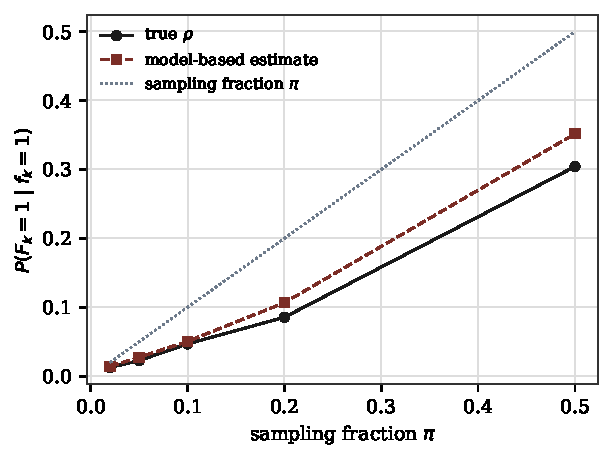
\includegraphics[width=0.62\textwidth]{fig5_journalist.pdf}
\caption{The uniqueness probability $\rho = \Prob(F_k = 1 \mid f_k = 1)$ against the
sampling fraction on the synthetic population: the truth (solid line, circles), the
model-based estimate from a fitted negative binomial law (dashed line, squares), and
the sampling fraction (dotted diagonal), which is not an approximation to $\rho$.}
\label{c11:fig-journ}
\end{figure}

Here the simulation shows something a formula could not, because the model's own
check fails. If the negative binomial law were right, the fitted dispersion would
be the same at every sampling fraction. It rises from 0.33 at $\pi = 0.02$ to 0.51
at $\pi = 0.2$ and 0.59 at $\pi = 0.5$.
% source: artifacts-paper/results.json, measures.journalist[*].dispersion (0.3251, 0.3799, 0.4407, 0.5051, 0.5944); paper/bis_ifc_full.tex line 1437
The drift is evidence of misfit, and the estimate of $\rho$ was conservative here by
good fortune, not by design. On a real file, where $\rho$ has no truth to be compared
with, the drift is the only warning available, which is why Part~VI includes a test
that fits the law at several subsample fractions and rejects it when the dispersion
moves.

Naledi kept this result in mind for the research file. Tomás's file was a sample,
the Bank knew its sampling fraction, and she could compute $\rho$. What she could
not do on the Bank's own data was check it. The simulation told her how far off a
fitted law could be on a population of this shape and which symptom to look for.

\section{Measurement error does not simply reduce risk}

Practitioners usually expect errors in the adversary's information to reduce its
success, and the expectation is half right. Under exact exchangeable matching, the
predicted success for a uniformly drawn released target is the mean prosecutor risk,
0.4663. Simulating the declared adversary with its reporting errors on age band and
occupation, but without the covariate, gives 0.3812 over 5,000 replicates. That is
the reduction practitioners expect.
% source: paper/generated/numbers.tex (\runattacktheory 0.4663, \runattackkeyonly 0.3812); artifacts-paper/results.json attack.key_error_trials 5000

Adding the single noisy reading of $y$ returns the success rate to 0.4642 over
20,000 replicates, with a one-sided 95 per cent upper bound of 0.4701.
% source: paper/generated/numbers.tex (\runattackcovariate 0.4642, \runattackupper 0.4701); artifacts-paper/results.json attack.trials 20000
The reciprocal-frequency figure is therefore close to the truth for this release,
but by cancellation between an error that spreads the posterior across candidates
and a covariate that concentrates it on one. An assessment that modelled only the
reporting error would have understated the risk by 18 per cent.
% source: paper/generated/numbers.tex \runattackunderstatement 18

The formulas of Chapter~\ref{ch:scenario} said that both effects exist and that
their net direction is open. They could not say that on an ordinary file the two
nearly cancel, so that a practitioner who uses the reciprocal frequency is right by
accident, and one who corrects it for reporting error alone is wrong by a fifth.
That is the second thing the simulation adds: the direction and size of effects that
the formulas leave open.

The same run tests the adversary's posterior itself. Figure~\ref{c11:fig-calib}
groups the targets by the maximum posterior the adversary computed and plots, for
each group, the share of its guesses that were right. When the adversary's model
matches the process that generates its information, the mean gap between the binned
posterior and the empirical success rate is 0.007. When the adversary assumes a
covariate 2.5 times noisier than the truth, the gap rises to 0.049, and the error
is one-sided: the posterior understates the success rate in the lower bins. The
overall success rate barely moves, from 0.4642 to 0.4571.
% source: paper/generated/numbers.tex (\runcalibrationgapcorrect 0.007, \runcalibrationgapwrong 0.049, \runmisspecifiedrate 0.4571); artifacts-paper/config.json misspecified_covariate_factor 2.5

\begin{figure}[ht]
\centering
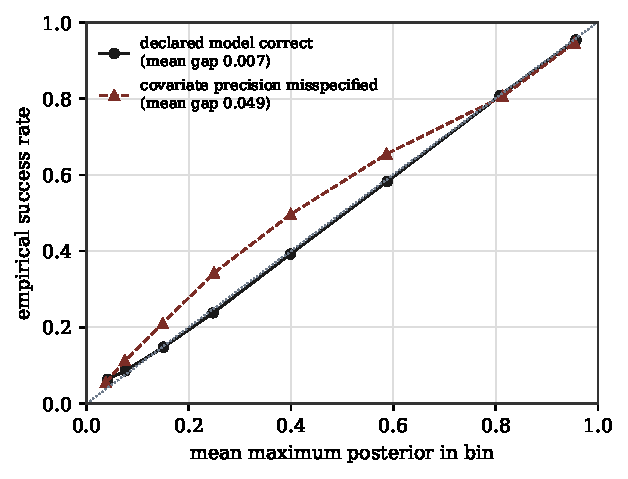
\includegraphics[width=0.58\textwidth]{fig3_calibration.pdf}
\caption{Calibration of the adversary's maximum posterior against the empirical
success rate, 20,000 replicates per curve: the declared model (solid line, circles)
and a model that misstates the covariate's precision (dashed line, triangles). The two models give overall success rates that
differ by 0.007, while their calibration gaps differ by a factor of seven.}
% source: paper/bis_ifc_full.tex, caption of fig:calib
\label{c11:fig-calib}
\end{figure}

The practical point is that a single risk number need not reveal that the linkage
model is wrong. Two models that disagree about the adversary's precision give the
same headline rate to two decimal places. A calibration check on matches whose truth
is known does reveal it, and the check needs exactly what a simulation on a known
population supplies. An institution cannot run it on its real file, but it can run
it on held-out records from its own data when it plants targets whose links it
knows, which is the first falsification test of Part~VI.

\section{$k$-anonymity does not deliver $1/k$}\label{c11:sec-kanon}

The chapter's opening fact comes from applying minimum class sizes of 3, 5, 10 and
20 to the declared key, suppressing records in smaller classes, and attacking what
remains. Two controls are measured, because they answer different questions. The
first is the average risk of a target drawn uniformly from the released records,
from 12,000 replicates. The second is the risk of the worst target among those in
the smallest released classes, each estimated from 250 replicates of its own and
reported with a lower bound that carries a correction for the selection.
% source: paper/generated/table_kanonymity.tex (caption and rows); artifacts-paper/config.json attack_replicates (kanon 12000, per_target 250)
The decision rule of Chapter~\ref{ch:decision} is stated for every target in a
declared set, so the second control is the one the rule needs.

Figure~\ref{c11:fig-kanon} shows both against the nominal bound $1/k$. The average
stays below $1/k$ at $k = 3$ and $k = 5$, at 0.2573 and 0.1852, and exceeds it at
$k = 10$ and $k = 20$, at 0.1129 and 0.0787. The worst target exceeds $1/k$ at every
level, and so does its corrected lower bound, which is 0.82, 0.78, 0.64 and 0.68 as
$k$ runs from 3 to 20. Between 27 and 75 per cent of the targets in minimum-size
classes have an individual lower bound above $1/k$.
% source: paper/generated/table_kanonymity.tex; paper/generated/numbers.tex (\runkanon*average, \runkanon*worstlowerprose)

\begin{figure}[ht]
\centering
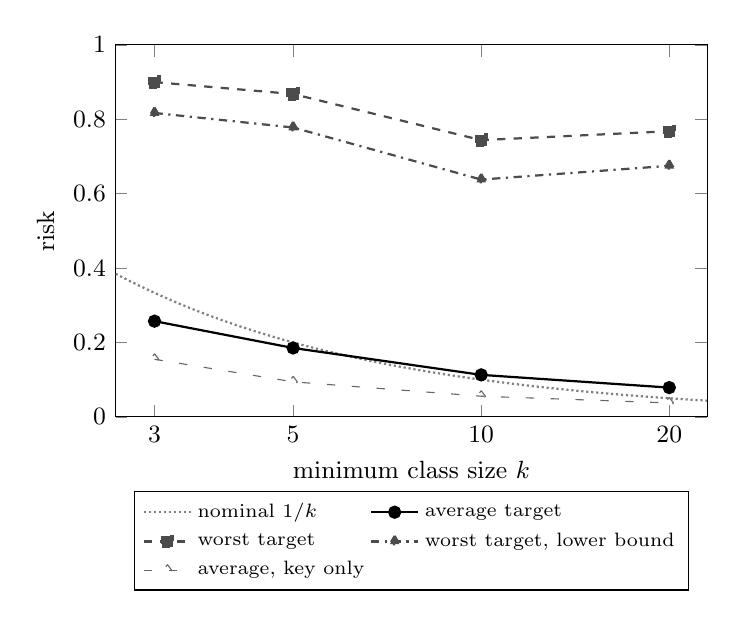
\begin{tikzpicture}
\begin{axis}[width=0.75\textwidth,height=0.52\textwidth,
  xmode=log, log basis x=10, xtick={3,5,10,20}, xticklabels={3,5,10,20},
  xmin=2.6,xmax=23, ymin=0,ymax=1,
  xlabel={minimum class size $k$}, ylabel={risk},
  legend style={at={(0.5,-0.2)},anchor=north,legend columns=2,font=\scriptsize}, legend cell align=left,
  tick label style={font=\small},label style={font=\small}]
\addplot[thick,black!50,densely dotted,mark=none,domain=2.6:23,samples=40] {1/x};
\addlegendentry{nominal $1/k$}
\addplot[thick,black,solid,mark=*] coordinates {(3,0.2573) (5,0.1852) (10,0.1129) (20,0.0787)};
\addlegendentry{average target}
\addplot[thick,black!70,dashed,mark=square*] coordinates {(3,0.900) (5,0.868) (10,0.744) (20,0.768)};
\addlegendentry{worst target}
\addplot[thick,black!70,dashdotted,mark=triangle*] coordinates {(3,0.817) (5,0.778) (10,0.638) (20,0.675)};
\addlegendentry{worst target, lower bound}
\addplot[thin,black!60,loosely dashed,mark=diamond] coordinates {(3,0.1548) (5,0.0942) (10,0.0555) (20,0.0375)};
\addlegendentry{average, key only}
\end{axis}
\end{tikzpicture}
\caption{Minimum class size against the simulated risk of the declared adversary on
the synthetic population. The worst target and its lower bound, corrected for
selection, stay far above the nominal bound $1/k$ at every level; the average
crosses it between $k = 5$ and $k = 10$. Without the reading of the continuous
variable (key only) the average stays below $1/k$. Series differ by line style and
marker as well as shade.}
\label{c11:fig-kanon}
\end{figure}
% source: paper/generated/table_kanonymity.tex (average, worst, bound); artifacts-paper/results.json k_anonymity[*].key_only (0.1548, 0.0942, 0.0555, 0.0375)

The lowest curve in the figure identifies the cause. The same adversary without its
reading of $y$ succeeds on average with probability 0.0555 at $k = 10$, below the
nominal 0.1, and stays below $1/k$ at every level.
% source: artifacts-paper/results.json, k_anonymity[k=10].key_only = 0.0555
The failure is a failure of key selection, not of the criterion. The covariate
separates members of a key class, and raising $k$ on a key that leaves it out
shrinks the share of the adversary's information that the criterion controls while
leaving the covariate untouched. One reading of why the average overtakes $1/k$ at
the larger levels is that the nominal bound falls in proportion to $1/k$ while the
covariate's power to separate the members of a class falls more slowly; the study
did not test this.

Proposition~\ref{prop:kanon} predicted that this could happen. The simulation shows
that it happens at every level of $k$ on a population with nothing contrived about
it, and that the size of the failure is not small: the worst record in a
20-anonymous release is identified about three times in four. That is the third
thing the simulation adds. Formulas about averages are silent about the worst
record, and the worst record is what a rule stated as a supremum must control.

The cost is as plain as the failure. Figure~\ref{c11:fig-riskdist} shows the
distribution of the formula's own risk $1/f_k$ across released records under each
minimum class size. Reaching $k = 10$ keeps 15.5 per cent of the released records,
and reaching $k = 20$ keeps 4.8 per cent.
% source: paper/generated/numbers.tex (\runkanon10retainedpct 15.5, \runkanon20retainedpct 4.8)

\begin{example}[The worst of 230 targets]\label{c11:ex-worst}
At $k = 10$ the study examined 230 targets in the smallest released classes and attacked
each 250 times. The worst was named in 186 of its 250 attacks, a rate of 0.744. Read as
if it had been chosen in advance, its one-sided 95 per cent Clopper--Pearson lower bound
is 0.695. It was not chosen in advance: it was picked for having the largest count among
230. Proposition~\ref{c11:prop-worst} therefore takes the bound at level
$0.05/230 = 0.000217$, which gives 0.638. The correction costs 0.057 of the bound, and
what is left is still more than six times the nominal $1/k$ of 0.1. Naledi put the
corrected figure in her note to the chair and the uncorrected one in a footnote, with a
line saying why the smaller number was the one to read.
\end{example}

A release governed by its maximum prosecutor risk alone is pushed towards
discarding most of its content, and against this adversary it still fails.

\begin{figure}[ht]
\centering
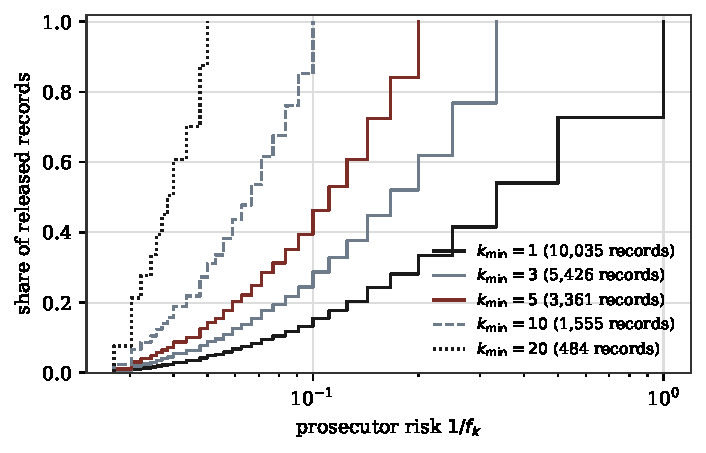
\includegraphics[width=0.66\textwidth]{fig1_risk_distribution.pdf}
\caption{Cumulative distribution of the prosecutor risk $1/f_k$ across released
records under minimum class sizes from 1 to 20, with the number of records each
keeps, as labelled in the legend. Governing the maximum of this measure
alone forces most of the file out of the release.}
\label{c11:fig-riskdist}
\end{figure}

The chair saw the figure at the next committee meeting and asked the question
Naledi had expected. If ten was not enough, what number was? Naledi's answer was
that no number on that key would do, because the variable doing the damage was not
in the key. The choices were to coarsen or perturb the borrowing measure, to leave
it out of the file, or to give Tomás access in the Bank's secure room, where the
question of linkage by an outsider did not arise in the same form.

\section{A programme of four releases}

Chapter~\ref{ch:programmes} used this population for its measurement of the pooling
gap, and the result needs only a short restatement here. Four releases from the same
sample, each keyed on ordinary demographic fields and each 3-anonymous, have
marginal risks between 0.0168 and 0.0884, so the marginals bound the chance that any
one release succeeds between 0.0884 and 0.2530. An adversary that intersects the
candidate sets of all four, through a record identifier the releases share,
succeeds with probability 0.4581, and 26.0 per cent of targets are identified
uniquely by the intersection although none was unique in any single release
(Figure~\ref{fig:pool-sim}).
% source: paper/generated/table_programme.tex; paper/generated/numbers.tex (\runprogrammelower, \runprogrammeunionupper, \runpooledall, \runpooleduniqueshare)

What the simulation adds to the proof is a test of whether the gap is an artefact of
the size of register chosen. Figure~\ref{c11:fig-scaling} rebuilds the same four
releases, with the same keys and the same minimum class size, on populations of
50,000, 100,000, 200,000 and 400,000 units with the sampling fraction held at 5 per
cent.

\begin{figure}[ht]
\centering
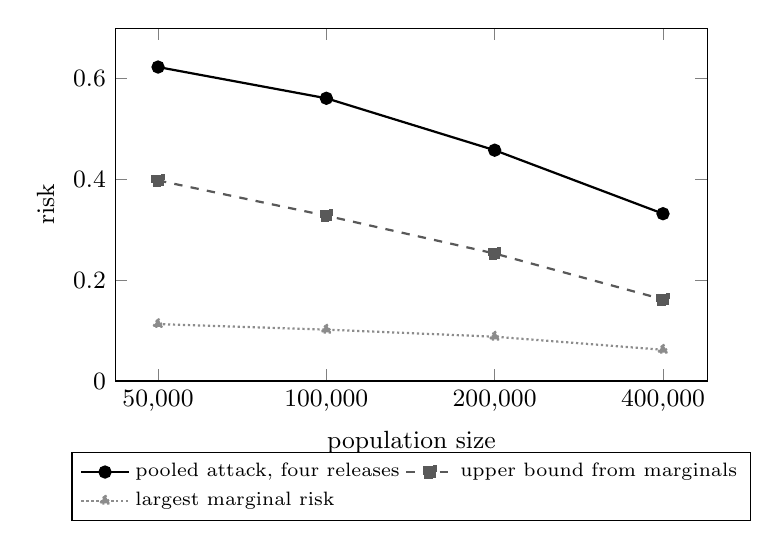
\begin{tikzpicture}
\begin{axis}[width=0.75\textwidth,height=0.5\textwidth,
  xmode=log, log basis x=2, xtick={50000,100000,200000,400000},
  xticklabels={50{,}000,100{,}000,200{,}000,400{,}000},
  xmin=42000,xmax=480000, ymin=0,ymax=0.7,
  xlabel={population size}, ylabel={risk},
  legend style={at={(0.5,-0.2)},anchor=north,legend columns=2,font=\scriptsize}, legend cell align=left,
  tick label style={font=\small},label style={font=\small}]
\addplot[thick,black,solid,mark=*] coordinates {(50000,0.623) (100000,0.561) (200000,0.458) (400000,0.332)};
\addlegendentry{pooled attack, four releases}
\addplot[thick,black!65,dashed,mark=square*] coordinates {(50000,0.398) (100000,0.328) (200000,0.253) (400000,0.162)};
\addlegendentry{upper bound from marginals}
\addplot[thick,black!45,densely dotted,mark=triangle*] coordinates {(50000,0.113) (100000,0.102) (200000,0.088) (400000,0.062)};
\addlegendentry{largest marginal risk}
\end{axis}
\end{tikzpicture}
\caption{The pooling gap at four register sizes, synthetic population, sampling
fraction 0.05, one draw per size. Each release becomes safer as the register grows,
and the pooled attack weakens more slowly than the bound the marginals imply, so the
ratio of the two rises from 1.57 to 2.05. Series differ by line style and marker.}
\label{c11:fig-scaling}
\end{figure}
% source: paper/generated/table_scaling.tex (all points; ratios 1.57, 1.71, 1.81, 2.05)

Two things move in opposite directions. Release by release, larger registers are
safer: the largest marginal risk falls from 0.113 to 0.062, because key classes grow
with the population. The pooled attack also weakens, but more slowly, so the ratio of
the pooled risk to the bound from the marginals rises from 1.57 at 50,000 units to
2.05 at 400,000.
% source: paper/generated/table_scaling.tex
Size does not dissolve the problem. It makes the marginals a worse guide to the
programme, the opposite of the reassurance a large register is usually taken to give.
One reading, which the study has not tested, is that growth adds records to every key
class, which protects each release, while the intersection of four candidate sets can
still close on one record.

Each size rests on one draw. At 50,000 units the Bernoulli sample gave 2,362 records
against an expected 2,500, about 2.8 standard deviations low, and that row should be
read with this in mind.
% source: paper/generated/table_scaling.tex (sample 2,362); paper/bis_ifc_full.tex, Appendix "Further simulation results" (2.8 standard deviations)
A register of several million would need its own run; the pipeline supports it by
changing one number in the configuration. That is the fourth and fifth thing the
simulation adds: it sizes the programme effect, and it shows how the size moves with
a design choice the proof does not contain.

\section{What the simulation says about its own uncertainty}

A simulation is itself an estimate, and Chapter~\ref{ch:estimate} separates two
sources of its error: the Monte Carlo error from a finite number of simulated
attacks, which the binomial interval describes, and the variance carried by the
sample and the fitted inputs, which it does not. The synthetic population allows the
separation to be measured. In a nested design, 120 outer replicates redraw the 5 per
cent sample from the same population, apply the same mechanism, and run 500 attacks
each. The within-replicate standard deviation is 0.0112. The between-replicate
standard deviation comes out at 0.0000 after correction, and the standard error of
the mean is 0.0010 whether the design term is included or not. The interval for the
share of variance the design contributes runs from 0 to 0.19.
% source: paper/generated/numbers.tex (\runnestedouter 120, \runnestedwithinsd 0.0112, \runnestedbetweensd 0.0000, \runnestedse 0.0010, \runnestedsharehigh 19); paper/bis_ifc_full.tex Appendix "How much the binomial interval misses" (500 attacks)

The binomial interval is adequate on this design, then, and the data could not have
told a design contribution of up to a fifth from none. Three features keep the term
small: the population is fixed and large, the sampling fraction is modest, and the
adversary's model is not refitted between replicates. None of the three is
guaranteed in practice. The simulation also measured how much worse the more capable
adversary does. Across the 45 settings of the protection grid of
Chapter~\ref{ch:tolerance}, the adversary with the twice-as-precise reading always
attains the larger risk, from 1 to 76 per cent above the declared one, with a median
gap of 40 per cent.
% source: paper/generated/numbers.tex (\rungridsettings 45, \runstresslow 1, \runstresshigh 76, \runstressmedian 40)
A risk figure reported for one adversary therefore carries an uncertainty about the
adversary that is far larger than its Monte Carlo error, and the record must say
which adversary it assumed.

The repository holds one further synthetic benchmark, for the multiscale extension
of the model that proposes protection settings in Chapter~\ref{ch:proposals}. It
uses its own seed and a deliberately nonlinear synthetic law with 400 training, 150
validation and 150 test rows, and reports held-out counted log losses of 0.2452 for a
linear model, 0.2252 for a deep model on raw inputs and 0.2247 for a deep model on
multiscale features.
% source: docs/MULTISCALE_MATHEMATICS.md (seed 30926; 0.24522193, 0.22520334, 0.22473617)
These are one-seed results on a law built to reward nonlinearity. They do not test a
release, they do not establish an advantage on real data, and they belong with the
proposal models of Chapter~\ref{ch:proposals}, which reports them in that context.

\section{What the simulation shows}

The chapter asked what an attack simulated on a known population shows that the
formulas cannot. The answer is that the formulas are statements of sign and
possibility, and the simulation turns them into statements of size on a population
of a stated shape. The formulas said that conventional measures are ordered; the
simulation found them spread across two orders of magnitude on one file. The
formulas said that measurement error could move risk either way; the simulation
found that on an ordinary file a reporting error and a single covariate nearly
cancel, so that the familiar formula is right by accident and its obvious correction
is wrong by a fifth. The formulas said that $k$-anonymity can fail once the adversary
reads a published continuous variable; the simulation found that it fails at every
level tried, with the worst record's lower bound more than six times $1/k$ at
$k = 10$ and $k = 20$, and that the failure disappears when the covariate is
removed.
% derived: 0.638/0.1 = 6.4 and 0.675/0.05 = 13.5, from paper/generated/table_kanonymity.tex The formulas gave the uniqueness
probability a model; the simulation found the model's own check failing. And the
proof of Chapter~\ref{ch:programmes} said that marginal risks cannot bound a pooled
attack; the simulation found that the gap widens as the register grows.

None of this replaces an assessment of a real release. Every number in the chapter is
conditional on a synthetic population whose parameters were chosen. What the
simulation supplies is the knowledge of which formulas to distrust, by how much, and
which symptoms to look for when no truth is available. Naledi's plan for Tomás's file
took that form. She would not simulate the Bank's population, which she could not
observe. She would plant known links among the Bank's own records, test the
adversary's calibration on them, fit the frequency law at several fractions, and
report the worst-record bound with its selection correction. When Grace read the file
a year later, the record named the adversary, the borrowing measure as the variable
that defeated the class-size rule, and the decision to release that measure only in
bands.

\begin{inpractice}[In practice: what to simulate before a release]
Simulate the declared attack whenever the release publishes a variable outside the
key that an adversary may also know, and report the worst-record bound with a
correction for selection, beside the average. Run the attack with and without each
auxiliary field to see which field drives the risk; if the risk is driven by a field
outside the key, raising the class size will not fix it. Check the adversary's
calibration on records whose links are known. If a frequency model is used for the
uniqueness probability, fit it at several subsample fractions and treat a moving
dispersion as a failed check. State the population, the seed and the parameters of
any synthetic study, and do not carry its numbers over to a real register.

\sloppy\smallskip\noindent\textit{In the software.} The population and its sample are built
by \texttt{privacy\_risk.synthetic} (\texttt{make\_register},
\texttt{apply\_mechanism}, \texttt{suppress\_small\_cells}). The attacks are in
\texttt{privacy\_risk.linkage} (\texttt{attack}, \texttt{per\_target\_risk},
\texttt{minimum\_cell\_targets}), the measures in \texttt{privacy\_risk.risk}, and the
selection-corrected bound in \texttt{uncertainty.selected\_maximum\_bound}. The
studies of this chapter are the functions \texttt{conventional\_measures},
\texttt{attack\_sequence}, \texttt{k\_anonymity}, \texttt{programme},
\texttt{programme\_scaling} and \texttt{design\_variance} in
\texttt{privacy\_risk.experiments}. The heart of the $k$-anonymity study is short:
\begin{lstlisting}
for minimum in config.get("kanonymity_levels", [3, 5, 10, 20]):
    mechanism = Mechanism(register.fine_band_width, register.occupations, int(minimum))
    release = apply_mechanism(register, mechanism)
    average = attack(register, release, model, replicates(config, "kanon", 12000),
                     np.random.default_rng(seed + 300 + minimum))
    targets = minimum_cell_targets(release, int(minimum), cap,
                                   np.random.default_rng(seed + 7))
    risks = per_target_risk(register, release, model, targets, reps,
                            np.random.default_rng(seed + 400 + minimum))
    worst = selected_maximum_bound(risks, reps, alpha)
\end{lstlisting}
\end{inpractice}

\section{Proofs}

The chapter states two results that its figures rely on.

\begin{proposition}[The uniform target]\label{c11:prop-uniform}
Under Assumptions~\ref{as:key} to~\ref{as:unif} of Chapter~\ref{ch:scenario}, the
success probability of an adversary attacking a target drawn uniformly from the $n$
released records is
\begin{equation}\label{c11:eq-uniform}
\frac{1}{n}\sum_{i \in I}\frac{1}{f_{K(X_i)}} = \frac{D_I}{n},
\end{equation}
where $D_I$ is the number of distinct keys in the release.
\end{proposition}

\begin{proof}
By Proposition~\ref{prop:recip}, a target with key $k$ is identified with probability
$1/f_k$, and a uniformly drawn target is record $i$ with probability $1/n$, which
gives the left side of \eqref{c11:eq-uniform}. Grouping the sum by key value, each
occupied key $k$ contributes $f_k$ terms each equal to $1/f_k$, so it contributes
exactly one, and the sum equals the number of occupied keys, $D_I$.
\end{proof}

\begin{proposition}[A lower bound for the worst selected target]\label{c11:prop-worst}
Let $T$ targets be attacked, target $j$ with $B$ independent replicates and success
count $K_j \sim \mathrm{Bin}(B, p_j)$, conditional on the release. Let $L_j$ be the
one-sided Clopper--Pearson lower bound at level $\alpha/T$, that is $L_j = 0$ if
$K_j = 0$ and otherwise the $\alpha/T$ quantile of the $\mathrm{Beta}(K_j, B-K_j+1)$
law. Let $\hat\jmath$ be any target chosen after seeing all the counts, for instance
the one with the largest $K_j$. Then
\[
\Prob\Bigl\{\, p_{\hat\jmath} \ge L_{\hat\jmath}\ \text{and}\ \max_j p_j \ge L_{\hat\jmath} \Bigr\} \ge 1 - \alpha .
\]
No independence between targets is needed.
\end{proposition}

\begin{proof}
First, each $L_j$ is a valid one-sided bound at level $\alpha/T$: for every $p_j$,
$\Prob\{L_j > p_j\} \le \alpha/T$. Write $\gamma = \alpha/T$ and
$G_p(k) = \Prob_p\{K \ge k\} = \sum_{s \ge k}\binom{B}{s}p^s(1-p)^{B-s}$. For
$k \ge 1$, $G_p(k)$ is continuous and strictly increasing in $p$, and the
binomial--beta identity gives $G_p(k) = I_p(k, B-k+1)$, so $L(k)$ is the unique $p$
with $G_p(k) = \gamma$. Hence $L(k) > p$ if and only if $G_p(k) < \gamma$, and this
set of counts is an upper tail $\{k \ge k^\ast\}$ because $G_p(k)$ decreases in $k$.
Therefore $\Prob_p\{L(K) > p\} = G_p(k^\ast) < \gamma$, or zero if the set is empty.

By the union bound,
$\Prob\{\exists j: L_j > p_j\} \le \sum_j \alpha/T = \alpha$, whatever the joint law
of the counts. On the complementary event every $L_j \le p_j$ holds at once, and in
particular $L_{\hat\jmath} \le p_{\hat\jmath} \le \max_j p_j$ for whichever target
was selected, since the selection only picks an index among inequalities that all
hold.
\end{proof}

Proposition~\ref{c11:prop-worst} is what licenses the figure of 0.638 at $k = 10$.
The correction divides $\alpha$ by the 230 targets examined, which costs width but is
needed: an uncorrected bound for the target with the largest observed count would be
biased upwards, because that target was chosen for having done well.
